\chapter{Motivations \& Evolution}

\paragraph{}
After talking about related works, we are going to list our motivations and then explain you the evolution of this project. 
\section{Motivations}
\paragraph{}
Social media has an important role in the real world and has an impact that was probably under-estimated a couple of years ago. Historical events like the arab spring or the election in Cambodia \cite{f_cambodia} are two examples that show how social media can be a powerful force for change when compared to other media. These events lead to studies about human behavior and engagement on these platforms.\\
For users, one of the main goals is to increase the time efficiency on social media. Today, you can see on Figure \ref{fig:clock} that 16 minutes per hour, or 27\% of each hour, spent online is on social media. There are many methods used to try to make users' time on social media more efficient.  As we saw with EdgeRank, the filtering of the information is one of the main ones.

\begin{figure}[h] 
\centering 
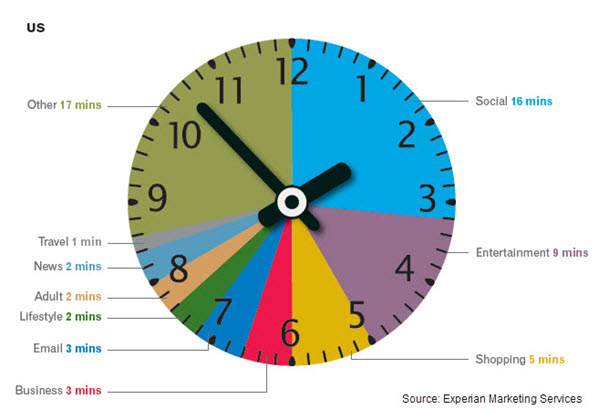
\includegraphics[width=0.6\columnwidth]{motiv/clock-time} 
\caption[Time spent of Social Media]{This clock shows the distribution of an hour online spent by US people. 16 min are on social network and forum. Source: \cite{s_clock}}
\label{fig:clock} 
\end{figure}

\paragraph{}
Recently, Twitter had to deal with an engagement problem. As we can see on Figure \ref{fig:engagement}, despite is 550 million users, Twitter has an engagement lower than Facebook or Instagram: this weakness led to  a drop in its stock price. However, "engagement" has no scientific definition and by consequence, there is no unique solution to this problem. By considering a new design which reduce the overload of information, it will be possible to analyse more details relating to the problem of engagement. By doing this it will be possible to improve user time efficiency and twitter engagement issues. \\

\begin{figure}[h] 
\centering 
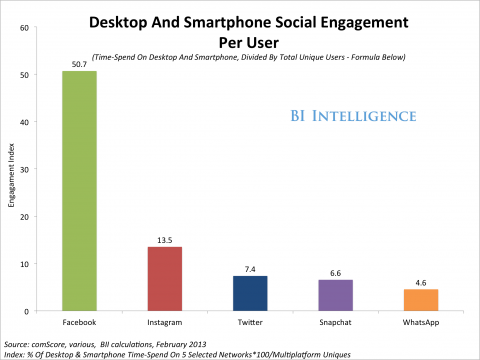
\includegraphics[width=0.8\columnwidth]{motiv/social-engag} 
\caption[Social Media engagement]{The graph gives us the social engagement per website. Facebook is from far the first one, it attracts roughly seven time more than Twitter. Source: \cite{s_engag_stats}}
\label{fig:engagement} 
\end{figure}

\section{Project evolution}
\paragraph{}
Information overload is a large topic and many aspects could have been approached. By viewing Table \ref{tab:table_analysis} can understand better why it was decide to focus the research on Twitter. Our three main criteria are: privacy, content and technique. Firstly, with Gmail, privacy and content were being dealt with. Due to the email variate and the personal characters of email, it was difficult to establish a protocol in order to improve the filtering of the emails.Secondly, we started to develop, with a similar design, applications based on different social media like Reddit or Tumblr. Finally, Tinder and Twitter were found to be of particular interest, due to the design of the Tinder app and the 140 character limit of Twitter. For these two reasons and Twitter's simple API The idea of Twinder was arrived upon.\\
You can find in annex the diagram \ref{fig:a_diagram} showing the evolution of the project through three aspects: technique, apps implementation and research.\\

\begin{table}[tb] 
\centering 
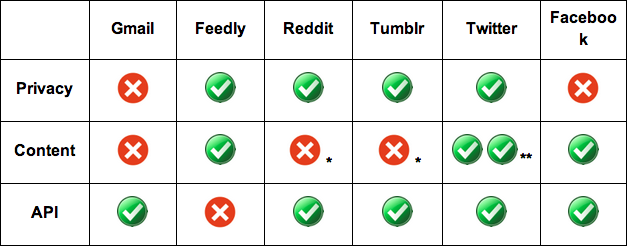
\includegraphics[width=1\columnwidth]{motiv/table_analysis} 
\caption[Social Media comparison]{In order to pick the best platform, we did a revue of 6 websites based on three criteria which are: privacy, content and API. \\
You can find the explanation below: \\
\textbf{Red}: problem for implementing the experiment. \\
\textbf{Green}: ok for implementing the experiment. \\
\textbf{*} : content is not constant. \\
\textbf{**} : 140 char with image or not. \\
}
\label{tab:table_analysis} 
\end{table}


